\title{Syllabus for A History of Science in Latin America: INTD262}
\author{Dr. Jordan Hanson - Whittier College Dept. of Physics and Astronomy}
\date{\today}
\documentclass[10pt]{article}
\usepackage[margin=1.5cm]{geometry}
\usepackage{outlines}
\usepackage{hyperref}
\usepackage{graphicx}
\begin{document}
\maketitle

\begin{abstract}
The scientific attitude exists in all human cultures, as does the desire to understand the natural world.  This course focuses on the scientific, medical, mathematical, and engineering practices of the Maya, Aztec, Inca, Colonial, and Modern Latin American civilizations.  The scientific evolution covered in this course begins in the 1700s, when Mayan, Aztec, and Incan scientific practices were combined with the principles of the European Enlightenment by Latin American Creoles.  Independence from Spain and Portugal were secured in the 19th century.  This nationalist transition was closely connected to the freedom to create scientific progress, and to spread modern education throughout Latin America.  Science and technology became omnipresent in 20th century Latin America, as it did in the United States and Europe.  In this course, we will first develop a historically-motivated definition for the scientific attitude.  Next, we will engage with the history of Latin American science through detailed discussions of essays exploring natural history, medicine and public health, the Enlightenment, and contemporary physics and astronomy research.  Class sessions will include activities that illustrate and enhance our understanding of diverse topics, from pre-Columbian mathematics to research performed by Latinos and Latin American citizens. Finally, students will create digital stories that showcase pre-Columbian, Enlightenment period, and modern scientific research from Latin America.
\end{abstract}
\noindent
\textit{\textbf{Pre-requisites}: None} \\
\textit{\textbf{Course credits, Liberal Arts Categorization}: 3 Credits, CON2/CUL4} \\
\textit{\textbf{Regular course hours and location}: Tuesday and Thursday, 11:00 am - 12:20 pm, SLC 311.} \\
\textit{\textbf{Instructor contact information}: jhanson2@whittier.edu (email), 918particle (Discord).} \\
\textit{\textbf{Office hours}: Please use the following link to schedule meetings: \url{https://fgucmvjkylvmgqfsco.10to8.com}.} \\
\textit{\textbf{Attendance/Absence}: Students needing to reschedule midterms must notify the professor a few days in advance.} \\ 
\textit{\textbf{Late work policy}: Late work is generally not accepted, but is left to the discretion of the instructor.} \\
\textit{\textbf{Course texts}: (1) ``Science in Latin America: A History,'' edited by Juan Jos\'{e} Salda\~{n}a.  (University of Texas Press, 2006). (2) ``The Scientific Attitude,'' by Lee McIntyre. (The MIT Press, 2019).} \\
\textit{\textbf{Grading}: The course grade will be a weighted average of assignment scores, and the weights are listed in Tab. \ref{tab:grades}.}
\begin{table}
\centering
\begin{tabular}{| c | c | c |}
\hline
\textbf{Assignment} & \textbf{Weight} & \textbf{Date} \\ \hline
Activities, group discussions, and reading quizzes & 20 \% & Tuesdays and Thursdays, 11:00 am - 12:20 pm \\ \hline
First Midterm, Take-home style, Units 0-2 & 20 \% & October 21st, 2024 (submit via PDF on Moodle) \\ \hline
Essay on Discovery, Expedition, or Researcher & 20 \% & November 1st, 2024 (submit via PDF on Moodle) \\ \hline
Second Midterm, Take-home style, Units 3-5 & 20 \% & December 9th, 2024 (submit via PDF on Moodle) \\ \hline
Final Project: Digital Storytelling & 20 \% & December 3rd and 5th, 2024 \\ \hline
\end{tabular}
\caption{\label{tab:grades} These are the grade weights for each assignment. The final project will be 10-15 minute digital story created using WeVideo.  Whittier College will provide access and training for WeVideo.}
\end{table}
\noindent
\textit{\textbf{Grade Settings}: $\geq 60\%, <70\%$ = D, $\geq 70\%, <80\%$ = C, $\geq 80\%, <90\%$ = B, $\geq 90\%, <100\%$ = A. Pluses and minuses: 0-3\% minus, 3\%-6\% straight, 6\%-10\% plus (e.g. 79\% = C+, 91\% = A-).} \\
\textit{\textbf{ADA Statement on Disability Services}: Whittier College is committed to make learning experiences as accessible as possible. If you experience physical or academic barriers due to a disability, you are encouraged to contact Student Disability Services (SDS) to discuss options. To learn more about academic accommodations, email disabilityservices@whittier.edu, call (562) 907-4825, or go to SDS which is located on the ground floor of Wardman Library.} \\
\textit{\textbf{Academic Honesty:} \url{https://www.whittier.edu/policies/academic/honesty}} \\
\noindent
\textit{\textbf{Course Objectives}:}
\begin{itemize}
\item To develop skill in written and oral expression of technical ideas, including scientific writing
\item To develop an appreciation for the growth and evolution of science in Latin America
\item To develop a broad perspective regarding the practice of science in other cultures
\item To develop a detailed understanding of modern Latin American scientific research and its cultural value
\end{itemize}
\clearpage
\twocolumn
\textit{\textbf{Course Outline}:}
\begin{outline}[enumerate]
\1 \textbf{Unit 0}: The Scientific Attitude, Nomenclature, and pre-Columbian Botany, Biology, and Medicine
\2 The Demarcation Problem: the line between science and non-science
\2 Terminology from philosophy, the Catholic Church, geography and the Spanish and Portuguese viceroyalties, scientific notation and number systems, and vocabulary from Nahuatl and Spanish
\2 Reading and discussion:
\3 The Introduction and Chapter 1 of \textit{The Scientific Attitude}
\4 Examples of good science: developments in medicine in the 19th century
\4 Examples of scientific denialism, pseudo-science, and scientific fraud
\3 Chapter 1 of \textit{Science in Latin America}
\4 Examples of botany, zoology, and herbal medicine of indigenous Mexican people (1600-1700)
\4 Comparisons to the knowledge of colonials, medieval medicine and the theory of the four humours
\4 Examples of transmission of knowledge: Europe to Latin America, and Latin America to Europe
\2 In-class group activities
\3 The Mayan numeric system, comparitive mathematics
\3 Classification of studies: science or non-science?
\3 Classification of species: hummingbirds
\3 Medicine: uses of \textit{s\'{a}bila}, or aloe vera, and anti-malarial and its treatmeant with quinine
\1 \textbf{Unit 1}: The Scientific Attitude, Pre-Columbian Mathematics, and the Application of Enlightenment Physics, Astronomy, and Chemistry to Public Progress in Nueva Espa\~{n}a and other \textit{virreinatos}
\2 Number systems and scientific notation
\2 Methods of computation pre-Columbian Latin America
\3 The Mayan number system, calendars and astronomical calculations
\3 The Quipu (Incan Empire), base 10 number systems, data representation
\3 Latin American contribution to the understanding of the solar system
\2 Reading and discussion:
\3 Chapters 2 and 3 of \textit{The Scientific Attitude}
\4 Misconceptions about science, identifying bad science
\4 Essential characteristics of good science
\3 Chapter 2 of \textit{Science in Latin America}
\4 Explanations for the adoption of Enlightenment scientific practice in Nueva Espa\~{n}a, Nueva Granada, Per\'{u}, and R\'{i}o de la Plata
\4 Scientific textbook shipments from France
\4 The creation of the Sociedades, Amigos del Pa\'{i}s, \textit{et cetera}, mining guilds, and scientific publications
\4 Formation of new institutions of higher education
\4 Applications of Enlightenment science in Latin America: mining practices, cartography, medicine, and astrophysics
\2 In-class group activities
\3 The Catholic Church and Education: mapping when The Society of Jesus (Jesuits), the Dominican Order of Preachers (OP), and Scholasticism or Enlightenment practice occupied an institute of higher learning
\3 Galileo, Kepler, and the heliocentric universe: verifying Kepler's Laws with evidence and Isaac Newton's theory of gravity
\3 Fr. Jos\'{e} Antonio Alzate y Ramírez and the story of the \textit{aurora borealis}.  Correspondence between Mexico and Northern Europe, and examples of American pseudo-scientific explanations
\3 Connection to modern physics research: Milagro, HAWC, and SWGO
\1 \textbf{Unit 2}: The Scientific Attitude, and the Teaching of Enlightenment Physics, Astronomy, and Chemistry in Nueva Granada and Per\'{u}
\2 Reading and discussion:
\3 Chapters 4 and 5 of \textit{The Scientific Attitude}
\4 Technical issues: the scientific attitude and the full demarcation problem
\4 Practical ways to embrace the scientific attitude
\3 Chapters 3 and 4 of \textit{Science in Latin America}
\4 Formation and evolution of institutions of higher education, competition between the Jesuits and Dominicans
\4 The creation of the Sociedades, Amigos del Pa\'{i}s, \textit{et cetera}
\4 Real Expedici\'{o}n Bot\'{a}nica del Nuevo Reino de Granada
\4 Aportes de Padre Jos\'{e} Celestino Mutis
\2 In-class group activities
\3 Comparing solar system models: Biblical, Ptolemaic, Copernican, and modern
\3 Mapping the timeline of scientific journals in Nueva Espa\'{n}a, Nueva Granada, and Per\'{u}
\3 Catching the scientific error: comparing climate science debate to the geocentric/heliocentric debate
\1 \textbf{First Midterm} - due October 21st, 2024
\2 The midterm will be posted on Moodle on Friday, October 18th.
\2 The exam will be completed at home, with an open-book/open-note policy.  The format is multiple choice, with some writing exercises.
\2 The exam is due in PDF form on Monday, October 21st, to be submitted via Moodle.
\begin{figure}[hb]
\centering
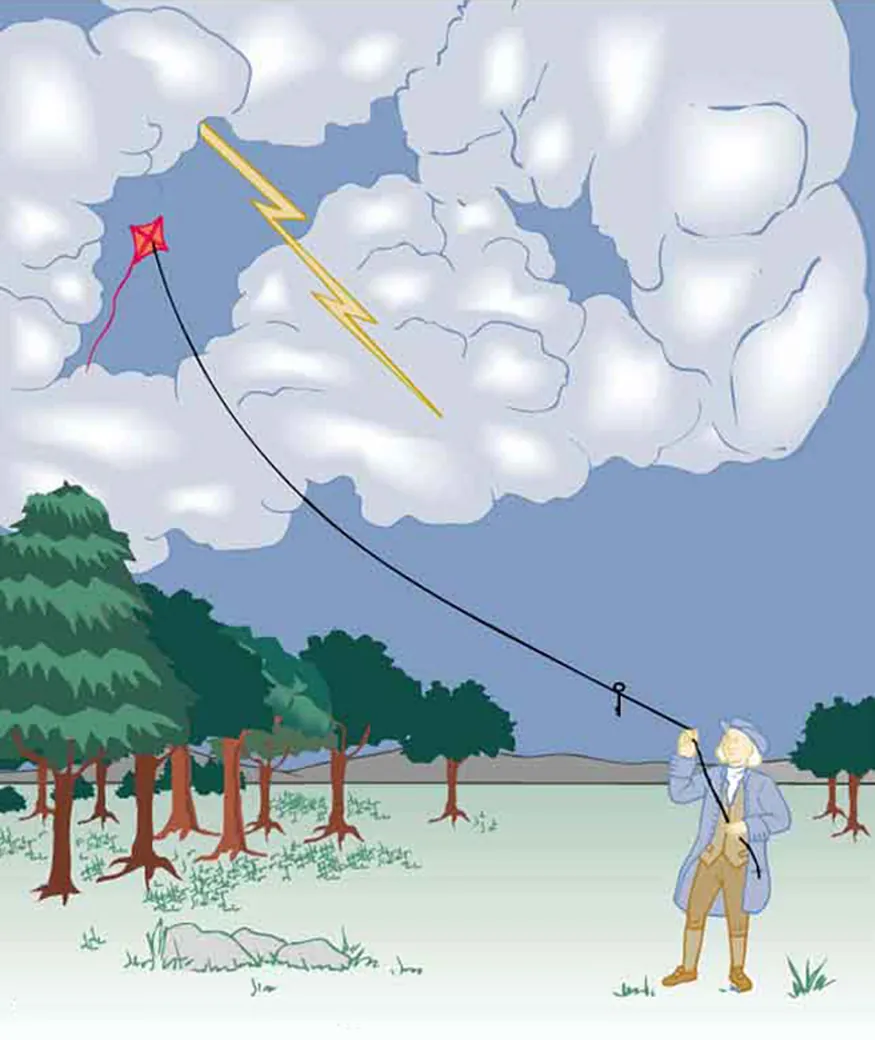
\includegraphics[width=0.20\textwidth]{figures/franklin.png}
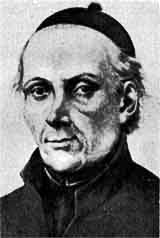
\includegraphics[width=0.15\textwidth]{figures/alzate_ramirez.jpg} \\
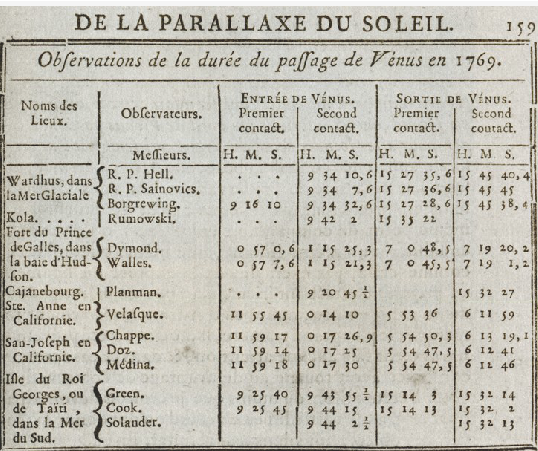
\includegraphics[width=0.40\textwidth]{figures/1769_transit.png} \\
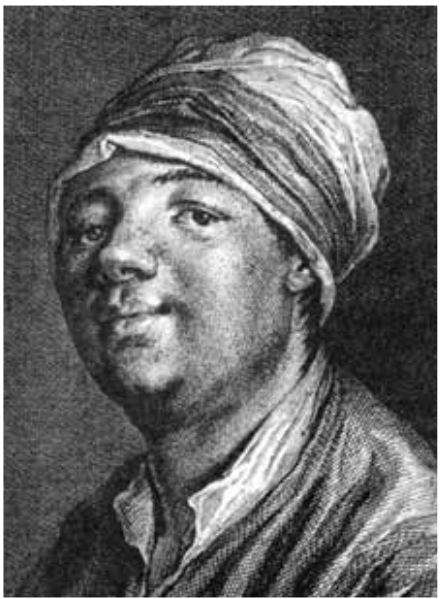
\includegraphics[width=0.175\textwidth]{figures/Abbot_dAuteroche.png}
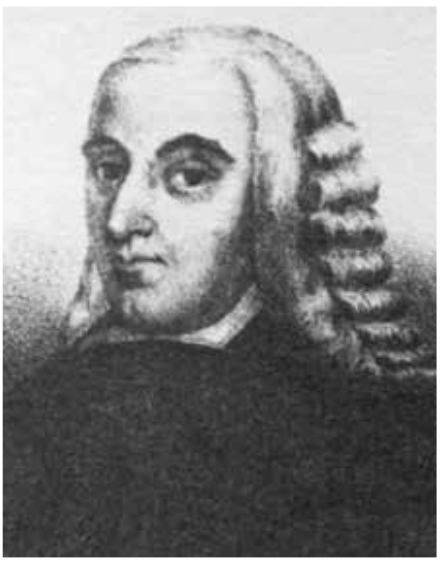
\includegraphics[width=0.175\textwidth]{figures/joaquin_v_d_Leon.png}
\caption{\label{fig:franklin} (Top left) Benjamin Franklin, (Top right) Father Jos\'{e} Antonio Alzate y Ram\'{i}rez, (Middle) Astronomical data from 1769 Venus transit, (Bottom left) Jean-Baptiste Chapp\'{e} d'Auteroche, (Bottom right) Joaqu\'{i}n Vel\'{a}zquez de Le\'{o}n.}
\end{figure}
\1 \textbf{Unit 3}: Applications and illustration
\2 Geographical calculations and analytical geometry (vectors and trigonometry)
\3 Latitude and longitude
\3 Triangulation and distance
\3 Kepler's Laws and planetary motion
\3 The optical obervatories of the Andes mountain range
\2 Atacama Large Millimeter/submillimeter Array (ALMA)
\2 Pierre Auger Observatory (PAO)
\2 Brief remarks about \textit{History and Current Status of Modern Science in Antarctica}: learning from indigenous science and technology
\1 \textbf{Essay on Discovery, Expedition, or Researcher} - due November 1st, 2025
\2 Format: essays will be approximately 5,000 words, and can be enhanced with figures, diagrams, maps, and charts.
\2 Protocol: submit via PDF on Moodle
\2 Editing/drafts: please use the booking link (above in contact info) to schedule office hours appointments.  Students can use these appointments to improve the content and structure of the paper.
\2 \textbf{Prompt:} ``Select a major Latin American scientific discovery, expedition, or researcher.  Using the course texts and bibliographies within them, expand upon the scientific history of the discovery, expedition, or researcher.  Include the historical context of the work, the methodology, and the important results of the work.''
\1 \textbf{Unit 4}: Modern Science and Nationalism in Latin America during the 1800s
\2 Scientific progress was part of the origin story for Latin American nationalism
\2 Analysis of Constitutions and Laws from Latin America in the 1800s
\2 Reading and discussion:
\3 Chapter 5 of \textit{Science in Latin America}
\4 When the Creole elites decided to break away from Spain and Portugal
\4 Achieving economic, educational, and medical reforms
\4 Examples of the participation of leading scientists in revolutionary activities
\3 Chapter 6 of \textit{The Scientific Attitude}
\4 These discussions center on the state of medicine in the 1800s
\4 The history of progress in medical sciences connects to Unit 5
\2 In-class group activities
\3 Build a university: (a) structure the curriculum, (b) assess the numbers and variety of required texts and (c) courses to be taught, and (d) estimate the time and cost to assemble minimum academic materials, students, and professors.
\3 Design a constitution: (a) demarcate government structures from the people, (b) select which social activities or rights shall be explicitly enumerated, versus implied, and (c) determine the internal structure of government branches.
\1 \textbf{Unit 5}: Development of Latin American Medicine
\2 Review of pre-Columbian and Medieval European medicine
\2 Final project discussions: family medicinal practices, developments in \textit{traditional medicine}
\2 Final project discussions: developments in Latin American physics and astrophysics
\2 Reading and discussion:
\3 Chapters 6 and 8 of \textit{Science in Latin America}
\4 Developments in anatomical and clinical medicine
\4 Developments in microbial research and laboratory based medicine
\4 History of excellence in biomedical research in Latin America
\3 Chapters 7-9 of \textit{The Scientific Attitude}
\4 Science gone wrong, concepts of sin, fraud, denialism, and pseudo-science
\4 The scientific attitude in the social sciences
\2 In-class group activities
\3 Group reflection: is science possible without morality?
\3 Discussion: can the scientific attitude be applied without a moral framework?
\3 Experiences in traditional medicine
\1 \textbf{Second Midterm} - due December 9th, 2024
\2 The midterm will be posted on Moodle on Friday, December 6th.
\2 The exam will be completed at home, with an open-book/open-note policy.  The format is multiple choice, with some writing exercises.
\2 The exam is due in PDF form on Monday, December 9th, to be submitted via Moodle.
\1 \textbf{Final Project Presentations} - given in class on December 3rd and 5th
\2 Form groups of 2, or remain solo (students' choice).
\2 Select a topic different than the topic chosen for the mid-semester essay.
\2 Create a 10-15 minute digital story using WeVideo that illustrates the topic in a way that educates our peers.
\2 Students will receive training and access for the WeVideo tools, which Whittier College provides for free.
\2 Digital stories will be graded according to the following breakdown:
\3 For \textit{original} storytelling, filled with \textit{factually verifiable} content, 30\%.
\3 For \textit{clearly communicating} the content, including legibility and sensible graphics, 30\%.
\3 For \textit{meeting but not exceeding} the time-requirement with appropriate amount of content, 30\%.
\3 For \textit{articulating the idea with a unique style}, 10\%.
\end{outline}
\begin{figure}[hb]
\centering
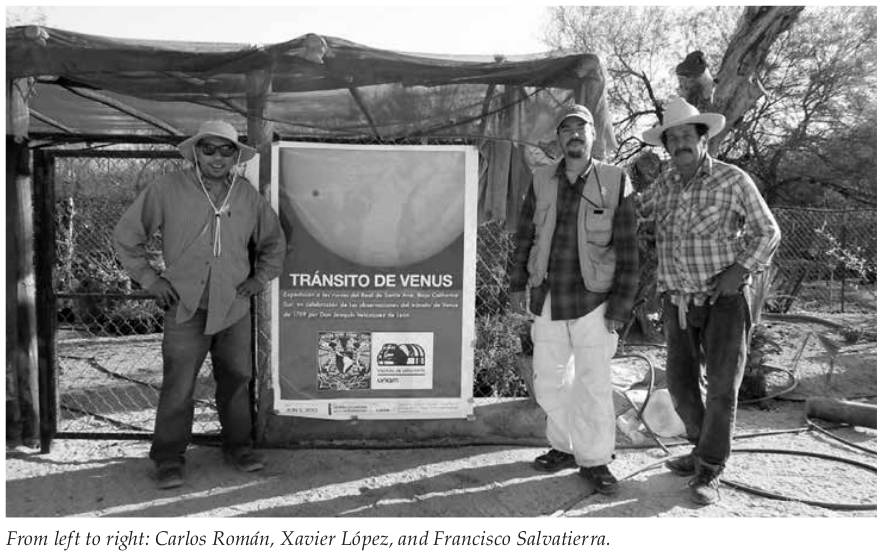
\includegraphics[width=0.45\textwidth]{figures/roman_lopez_salvatierra.png}
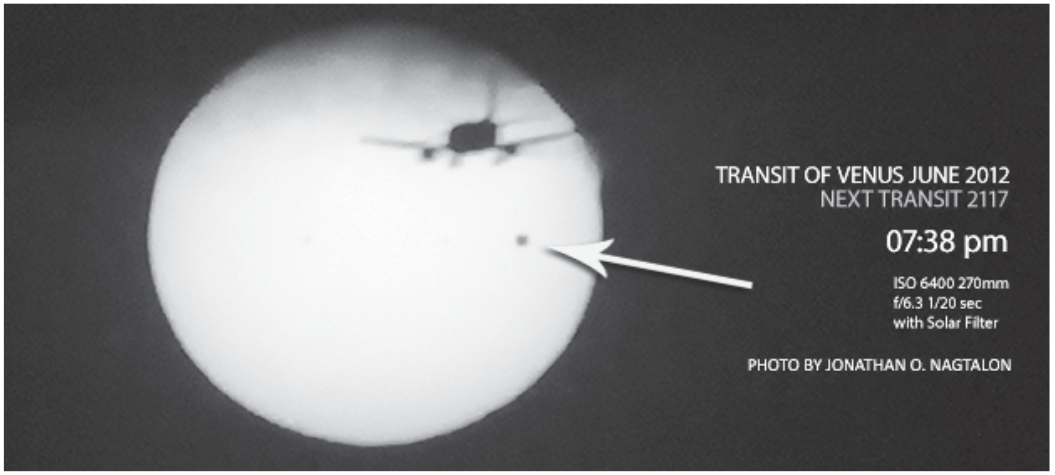
\includegraphics[width=0.45\textwidth]{figures/venus.png}
\caption{\label{fig:franklin2} (Top) Carlos Rom\'{a}n, Xavier L\'{o}pez, and Fransisco Salvatierra. (Bottom) The 2012 Venus transit, from Baja California.}
\end{figure}
\end{document}
